\documentclass[12pt]{article}

\usepackage{fullpage}
\usepackage{multicol, multirow}
\usepackage{tabularx}
\usepackage{standalone}
\usepackage{listings}
\usepackage{ulem}
\usepackage{amsmath}
\usepackage{pdfpages}
\usepackage[utf8]{inputenc}
\usepackage[russian]{babel}

\newcommand{\StudentName}{Ильвохин Дмитрий}
\newcommand{\Group}{1O-106М}
\newcommand{\CourseName}{Программирование игр}
\newcommand{\LabNum}{1}
\newcommand{\Subject}{Бильярд или шарики 2D}
\newcommand{\PrepName}{Аносова Н.\,П.}

\begin{document}

\lstset
{
        language=Python,
        basicstyle=\footnotesize,% basic font setting
        extendedchars=\true
}

\begin{flushright}
\Large{
	\CourseName \\
	Лабораторная работа №\,\LabNum \\
	<<\Subject>> \\
	\StudentName, \Group \\
}
\end{flushright}

\subsection*{Задание}
По левому клику мыши на свободном месте генерируется шарик случайного цвета,
повторный левый клик <<выделяет>> шарик. Правый клик мыши заставляет выделенные
шарики двигаться к месту клика, начальная скорость у всех шариков одинаковая,
при этом они <<развыделяются>> и приобретают первоначальный цвет.

В процессе движения шарики могут сталкиваться между собой, с неподвижными шарами
и краями окна, столкновение считать упругим.

Движение должно постепенно замедляться из-за силы трения.

Кроме того на шары действует очень слабая сила тяжести, заставляющая
их постепенно двигаться вниз.

По клавише <<пробел>> всю сцену можно <<встряхнуть>>.

\subsection*{Практическая часть}
Для реализации игры был выбран движок LÖVE (love2d) --- свободно распространяемый игровой движок,
предназначенный для написания компьютерных игр на языке Lua.

В отличие от многих популярных движков LÖVE не представляет и себя конструктор игр.
Для написания кода игры можно использовать любой текстовый редактор с подсветкой синтаксиса языка Lua.
Также в нём нет редактора уровней, все изображения, уровни и персонажи прописываются в коде игры.~\cite{love}

Это был мой первый опыт разработки на языке Lua, как впрочем и разработки
игор вообще. Но несмотря на это, разобраться получилось довольно быстро,
благодаря богатой официальной документации игрового движка и наличию
большого количества обучающего материала в сети.

Результат выполнения лабораторной работы можно увидеть на рисунке \ref{fig:game}.

\begin{figure}[!htb]
  \centering
    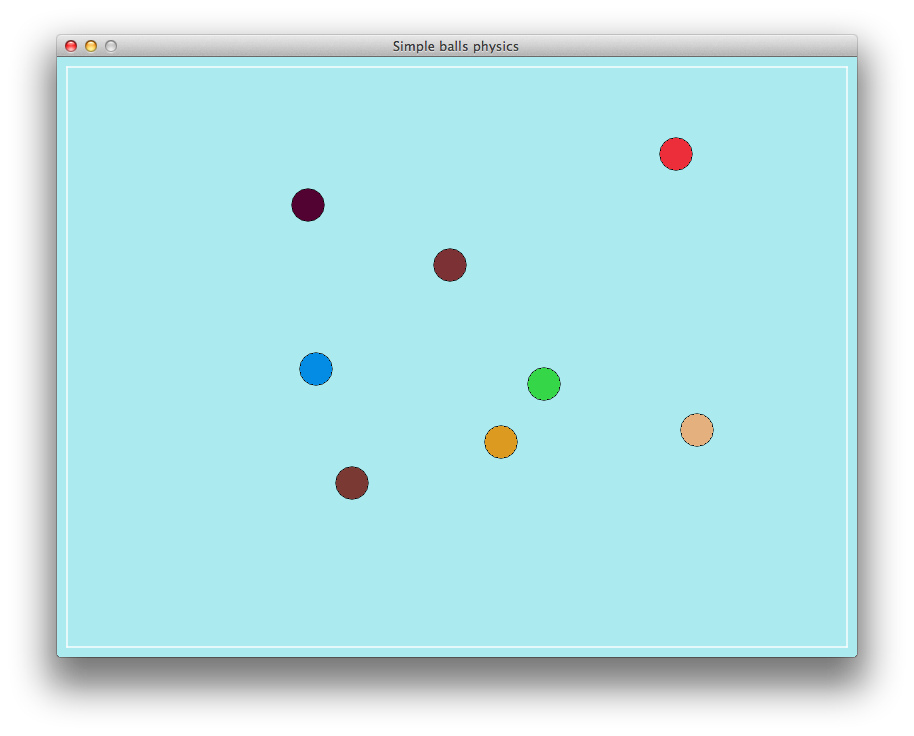
\includegraphics[scale=0.5]{pics/game.png}
   \caption{Скриншот из игры}
    \label{fig:game}
\end{figure}

\subsection*{Выводы}
Ничего особенного в реализации игры нет. Нужно было вспомнить немного 2D геометрии и основы
физики. С новым для меня языком Lua тоже не возникло особых проблем, хотя теперь могу сказать,
что некоторые вещи можно было сделать немного иначе, получилось бы и короче и яснее.

\begin{thebibliography}{}
\bibitem{love} https://ru.wikipedia.org/wiki/LÖVE
\bibitem{love_official} https://love2d.org/wiki/Main\_Page
\end{thebibliography}

\end{document}

